% Native publication source; requires tikz. Keep the coordinate list as a text equivalent.
\begin{figure}[htbp]
\centering
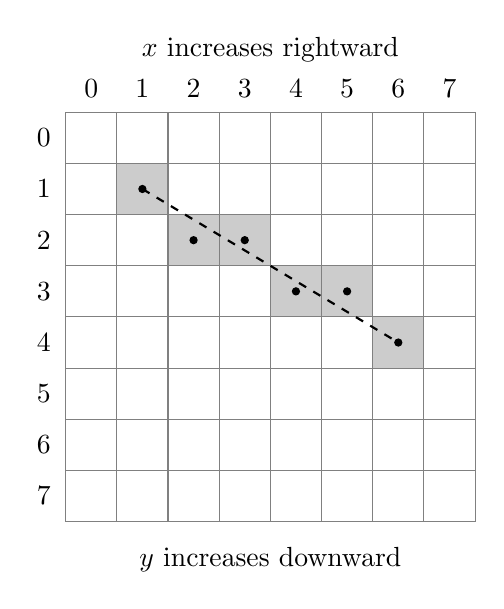
\begin{tikzpicture}[x=0.65cm,y=-0.65cm]
\foreach \x/\y in {1/1,2/2,3/2,4/3,5/3,6/4} {
  \fill[black!20] (\x-0.5,\y-0.5) rectangle (\x+0.5,\y+0.5);
  \fill (\x,\y) circle (1.5pt);
}
\foreach \k in {0,...,8} {
  \draw[gray] (\k-0.5,-0.5)--(\k-0.5,7.5);
  \draw[gray] (-0.5,\k-0.5)--(7.5,\k-0.5);
}
\draw[thick,dashed] (1,1)--(6,4);
\foreach \k in {0,...,7} {
  \node[above] at (\k,-0.6) {\k};
  \node[left] at (-0.6,\k) {\k};
}
\node[above] at (3.5,-1.3) {$x$ increases rightward};
\node[below] at (3.5,7.8) {$y$ increases downward};
\end{tikzpicture}
\caption{The line from $(1,1)$ to $(6,4)$. Shading and center dots identify selected cells; the dashed segment shows the continuous geometry.}
\label{fig:line-grid}
\end{figure}
